
\graphicspath{{./Images/Kapitel5/}}

	\section{Sensoren}
		\subsection{Übersicht} 
		
		In der vorliegenden Grafik (Fig.1) werden sämtliche Sensoren aufgezeigt:
			
				\begin{figure}
					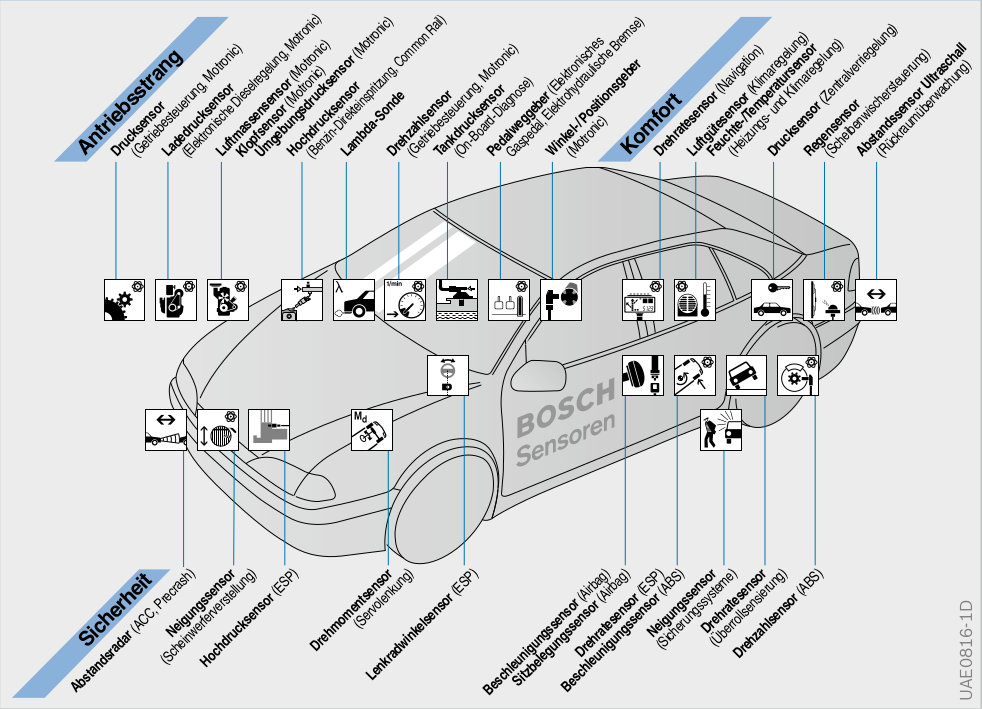
\includegraphics[width=15cm, height=11cm] {sensor_uebersicht.png}
					\caption{\cite{TS01}: Übersicht der Sensoren im Automobil}
				\end{figure}
			
		
			\begin{flushleft}	
			
			Für einen besseren Überblick werden in diesem Kapitel die Sensoren des Automobils begutachtet, aufgelistet und erläutert.	
			
			\end{flushleft}	
			
				\subsubsection{Begriffsdefinition}
					
					Unter Sensor versteht man im allgemeinen eine Komponente/ Fühler/ Detektor/ Aufnehmer, welche eine physikalische Größe oder chemische Effekte durch messtechnische Verfahren aufgenommen und in ein analoges, elektrisches Signal convertiert.

				\subsubsection{Arten}
				In folgender Tabelle (Table 1) sind diversen Arten von Sensoren aufgelistet:
					\begin{table}
						\tiny{		
							\begin{tabular} {c|c|c|c}
								
								\textbf {Sensorart} & \textbf{Messtechnik} & \textbf {Beispiele} & \textbf{Erfassungsart}\\
								\hline
								
								Resistiv & Eletrische Widerstandsänderung & Dehnungsmessstreifen \\
								&& Potentiometrische Sensoren &  mechanisch\\
								
								
								\hline
								Induktiv & Änderung der Induktion & Schwingungsaufnehmer \\
								&& Induktivaufnehmer & nicht mechanisch\\
								\hline
								
								Wirbelstrom & Änderung des Wirbelstroms & Induktive Initiatoren & nicht mechanisch\\
								\hline
								
								Magnetfeld & Änderung des Magnetfelds & Hall-Generator\\
								&& Feldplatte & nicht mechanisch\\
								\hline
								
								Kapazitiv & Kapazitätsänderung & Drucksensor\\
								&& kapazitiver Näherungsschalter & mechanisch\\
								\hline
								
								Optoelektisch & Opto-elektrische Umsetzung & Fototransistor\\
								&& Fotodiode & nicht menchanisch \\
								\hline
								
								Temperatur & Kontaktthermometrie & Thermoelement\\
								&& Widerstandsthermometer & mechanisch\\
								
							
							\end{tabular}
							}
						\caption{ \cite{TS02}: Tabelle zur Einteilung von Sensoren}
					\end{table}
		
				

				\begin{flushleft}				
						Der Sensor erfasst also diverse physikalische Größen und durch die oben beschriebene Verfahren werden diese analog erfassten in analog- elektrische Strom-/ Spannungssignale umgewandelt.
						Hierbei kann man zwischen mechanischen und nicht mechanischen Sensoren unterscheiden.\\
						Unter mechanischen Sensoren versteht man, welche durch mechanische Einwirkungen ihren elektrische Eigenschaft verändern. Beispiele dafür sind Kraft oder Druckeinwirkung. Hierbei wird der Sensor mechanisch belastet.\\
						Nicht-mechanischen Sensoren unterscheiden sich soweit von den anderen, dass sie keine mechanische Einwirkungen brauchen. Diese reagieren auf die Änderung, welche keine Krafteinwirkung benötigen, beispielsweise Helligkeit.\cite{TS03}\\
						Des weiteren wird zwischen aktiven und passiven Sensoren unterschieden. Ein aktiver Sensor ist selbst ein Spannungserzeuger und benötigt keine weitere elektrische Hilfsenergie, um betrieben zu werden. Beispiele dazu wären ein Thermoelement, Licht- und Drucksensor.\\
						Passive Sensoren hingegen benötigen eine aktive Spannungsversorgung, auch Sekundärelektronik genannt, welche es erlaubt, die Messung in elektrische Signale, also in Primärelektronik, umzuwandeln. Beispiele dazu wären eine Wägezelle, Dehnungsmessstreifen, Magnetfeldsensoren.
						
						
				\end{flushleft}			
									
												
		\subsection{Klassische Sensoren im Automobil} 
		
			\begin{flushleft}
				In dem vorhergehenden Kapitel wurde ein grundlegendes Verständnis und eine grobe Eingliederung der Sensoren eingeordnet. Mit diesem Grundwissen wird im folgenden Kapitel auf Sensoren im KFZ- Bereich eingegangen.\\
				Grund für Sensortechnik im Automobil ist darauf zurückzuführen, dass sich im Laufe der Zeit sich das Automobil verändert hat im Hinblick auf Fahrunterstützung und Fahrhilfssysteme.
				Die Sensoren dienen hierbei der Eingabe von einem tatsächlichen Wert (Ist-Wert). Durch diese Angaben werden einer ECU (electronically controlled unit), also einer elektronischen Einheit via einem Bussystem gesendet, welche einen Abgleich des Ist-Wertes mit dem Soll-Wert errechnet und dementsprechend das Modul nachregeln und steuern kann. \\ 
				Da Sensoren diversen äußeren physikalischen und/ oder chemischen Einwirkungen ausgesetzt sind, müssen diese diesen entsprechend gerecht werden. Aus diesem Grund gibt es verschiedene Anfertigungsformen wie wasserdicht, dreck- und staubgeschützt. Diese werden in dem nächsten Kapitel ebenfalls erörtert.\\  
				
				Ein Ausfall des Sensors kann durch folgende Ursachen hervorgerufen werden
				\begin{itemize}
					\item Kurzschlussbegin
					\item Leitungsunterbrechung
					\item Verschmutzung
					\item Mechanische Beschädigung
					\item nicht korrektes Anbringen des Sensors
					\item Sensor defekt
				\end{itemize}	
				
				Nach einem Ausfall kann man durch gezielte Fehlersuche den Fehler analysieren:
				\begin{itemize}
					\item Anschlüsse prüfen
					\item Auslesen des Fehlerspeichers
					\item Allgemeine optische Prüfung
					\item Säubern der Sensoren
					\item Messungen mit einem Messinstrument vornehmen wie:
					\begin{itemize}
						\item Oszilloskop 
						\item Voltmeter
						\item Amperemeter
						\item Ohmmeter	
					\end{itemize}
					
				\end{itemize}					

				Nun werden die Sensor peu à peu erörtert. 



		\end{flushleft}	
		
			\subsubsection{Temperatursensor NTC}
				\begin{flushleft}
					Bei einem Temperatursensor handelt es sich um einen nicht-mechanischen, aktiver	Sensor, welcher die Temperatur erfasst.\\
					Die Sensoren sind auf einen Messbereich zwischen -40$^\circ$C und +200$^\circ$C skaliert ist. Ist die Temperatur über diesem Bereich werden spezielle Hochtemperatursensoren (HTS) verwendet.
				\end{flushleft}

				\begin{figure}
					\centering
					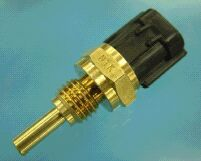
\includegraphics[width=5cm, height=4cm] {ntc.png}
					\caption{\cite{TS04}: Abbildung: NTC}
				\end{figure}
			
				\begin{flushleft}
						In der folgenden Abbildung (Fig. 2)wird der Aufbau eines Temperatursensors. Hierbei werden zwei unterschiedlich, elektrisch aufgeladene Metalle am Ende (der Messstelle) miteinander verbunden. Hier wird die Temperatur von dem zu messenden Element gemessen.\\
						Die Temperaturdifferenz wird an den zwei offenen Enden mit Hilfe des Seebeck-Effekts in elektrische Spannung umgewandelt. Nun kann man die Differenz der beiden Leiter vergleichen, wobei einer der Leiter als Referenz benutzt wird (grauer Leiter).\cite{TS05} 
						
				\end{flushleft}
					
				\begin{figure}
					\centering
					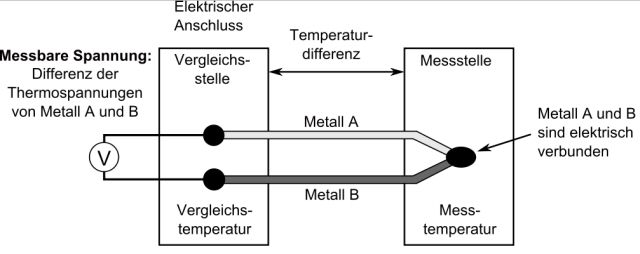
\includegraphics[width=12cm, height=6cm] {aufbau_ntc.png}
					\caption{\cite{TS06}: Abbildung: Aufbau NTC}
				\end{figure}
				
				\begin{flushleft}
					
					NTC Sensoren werden beispielsweise in folgenden Modulen angewandt:
					
					\begin{itemize}
						\item Katalysatorüberwachung
						\item Öltemperatur
						\item Klimaanlagen
						\item Kühlwassertemperatur 	
					\end{itemize}
					
					HTS hingegen werden für:

					\begin{itemize}
						\item AGR
						\item Turbolader
						\item Rußfilter 
					\end{itemize}
					eingesetzt.

				\end{flushleft}
		
			\subsubsection{Induktive Sensoren}
				
				\begin{flushleft}
					
					Diese arbeiten nach dem Induktionsgesetz. 
					Hierbei erleidet der Sensor keinerlei Verschleiß, da es keinen direkten Kontakt zu dem zu messenden Objekt existiert.\\
					Für ein Verständnis, wo diese Sensoren welche Aufgaben im KFZ- Bereich erfüllt, reicht es nur den groben Aufbau zu kennen.\\
					Eine Spule wird von Strom durchflossen, welche daraufhin ein Magnetfeld erzeugt.\\	
			
				\end{flushleft}		
			


				\begin{figure}
					\centering
					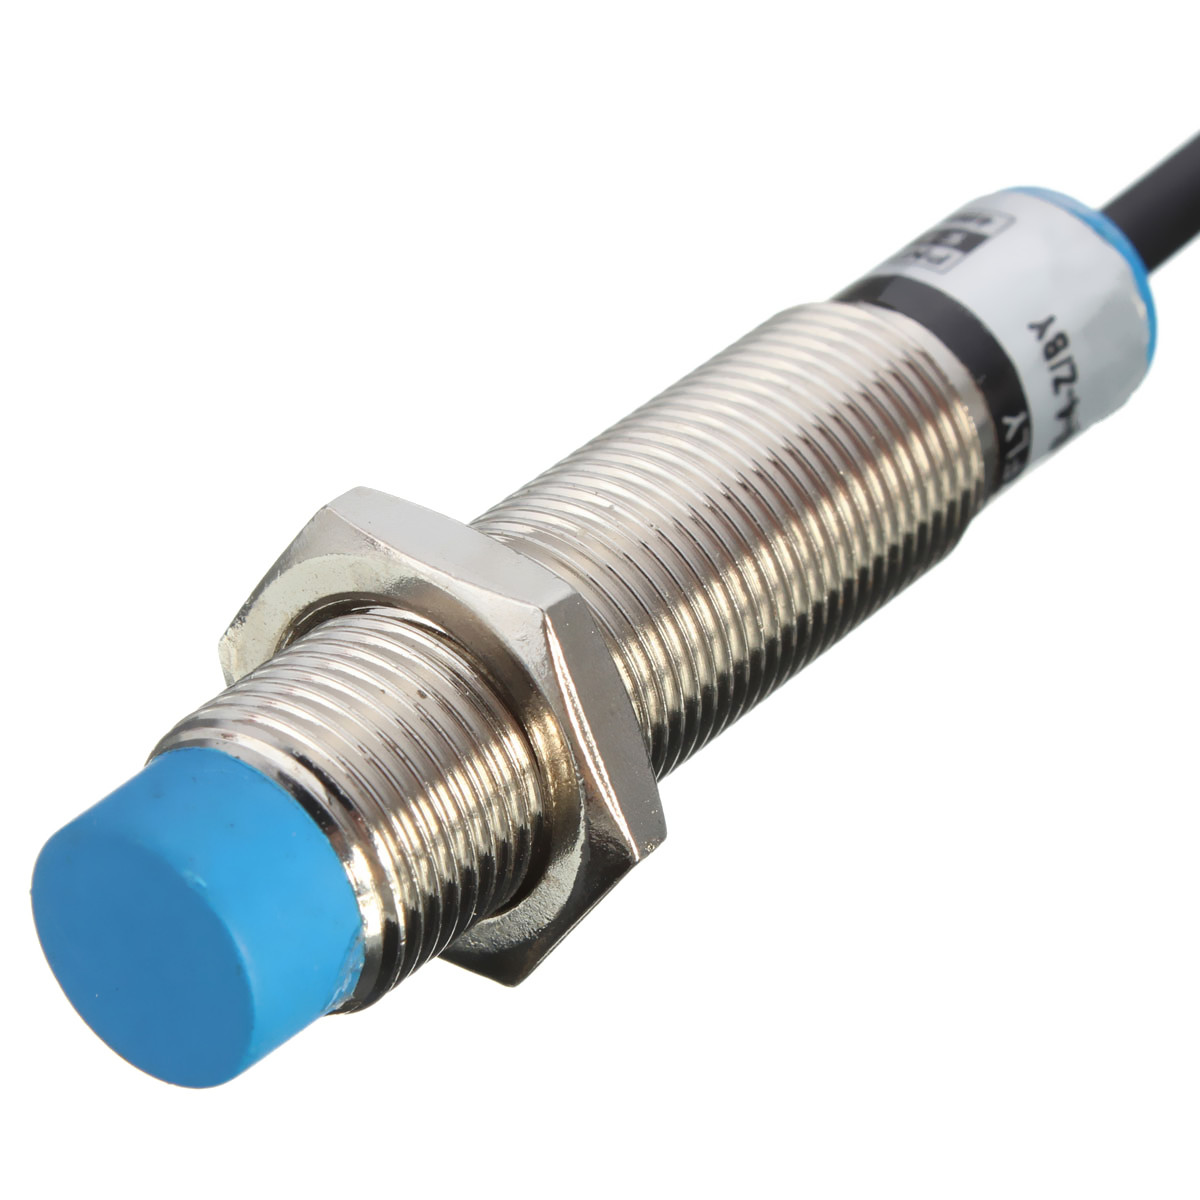
\includegraphics[width=5cm, height=5cm] {induktiv.png}
					\caption{\cite{TS07}: Abbildung: Induktiver Sensor}
				\end{figure}
			
			
				\begin{flushleft}
					In der Abbildung (Fig. 5) ist der Sensor über einer Art Zahnrad, welches man Impulsrad nennt, angebracht.\\
					"Der magnetische Fluss durch die Spule hängt davon ab, ob dem Sensor eine Lücke oder ein Zahn gegenübersteht. Ein Zahn bündelt den Streufluss des Magneten, eine Lücke dagegen schwächt den Magnetfluss." \cite{TS08}  
					Die Anzahl der Änderungen/ Impulse in einer bestimmten Zeiteinheit ist ein Maß für die Drehzahl des zu messenden Objekts. Darüber hinaus kann auch die exakte Position des Moduls erkannt werden.\\						
				\end{flushleft}
			
				\begin{figure}
					\centering
					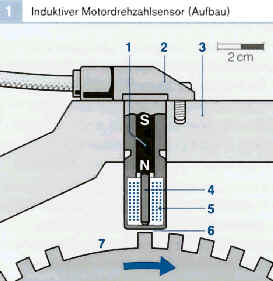
\includegraphics[width=7cm, height=7cm] {aufbau_induktiv.png}
					\caption{\cite{TS09}: Abbildung: Induktiver Sensor}
				\end{figure}
				
				\begin{flushleft}
					1 Dauermagnet, 2 Induktivgebergehäuse, 3 Motorgehäuse, 4 Weicheisenkern, 5 Induktionswicklung 6 Luftspalt, 7 Zahnlücken\\
					Induktive Sensoren werden beispielsweise in folgenden Modulen angewandt:
					
					\begin{itemize}
						\item Drehzahlerfassung wie
							\begin{itemize}
								\item Kurbelwellenstellung
								\item Getriebe
							\end{itemize}	
						\item Drosselklappenstellung
						\item Lenkwinkel z.b. ESP, "stear-by-wire"
						\item Fahrpedalgeber
						\item Bremspedal
					\end{itemize}
				
					Allerdings kann ein Ausfall eines Sensors zu erheblichen Schäden und sicherheitstechnischen Gefährdungen führen:
					\begin{itemize}
						\item Motor kann aussetzen oder gar stillstehen
						\item es wird ein Fehlercode abgespeichert
					\end{itemize}	
				\end{flushleft}				
		
			\subsubsection{Ölsensor}
				\begin{flushleft}
					
					Dieser Sensor wird verwendet, um den Zustand über des verwendeten Öls zu erhalten und den Füllstand. Somit kann angezeigt werden, wann ein Ölwechsel notwendig ist. Das Einbringen des Sensors spart also Geld, schont die Umwelt und gibt Rückschlüsse auf den Zustand des Motors und können Motorschäden verhindern.\cite{TS10}

				\end{flushleft}		
		
			\subsubsection{Lenkdrehmomentsensor}
				Um die Funktion des Servomoduls umsetzen zu können, benötigt das Steuergerät exakte Informationen über die vom Fahrer eingegebene Lenkbefehle. Um diese Eingabe richtig erfassen zu können, wurde ein Sensor konstruiert, welcher "[...]die erforderlichen Daten wie Drehwinkel, Drehrichtung und Drehmoment elektronisch erfassen.[...]"\cite{TS11} kann und an das Steuergerät sendet.\\
				Die Funktionsweise eines Drehmomentsensors kann durch zwei diverse Arten realisiert werden:\\
				
				\begin{itemize}
					\item 1. Magnetoresistives Prinzip:
							 Mittels Eingangswelle, Torsionsstab/ Drehstab (eine stabförmige Feder, welche sich in axialer Richtung drehen lässt), Antriebswelle und einem magnetoresisitem Element. \\
							 Damit Leitungen zur Spannungsversorgung und Signalübertragung nicht beschädigt werden, sind diese in einer Vermantelung, welche auch als Wickelkassette bezeichnet wird.\\ (Fig. 6)
							 
							 Durch das Einlenken des Fahrers wird der Torisonsstab ebenfalls verdreht. "Diese Verdrehung ist ein Maß für das Lenkmoment."\cite{TS12}\\
							 Durch gezieltes Aufbringen von Widerständen können die Drehbewegungen registriert werden. Durch das Drehen, also spannen oder stauchen der Feder ( Fahrer lenkt links bzw rechts ein) verändert sich das Megnetfeld, welches wiederum den elektrischen Widerstand verändert und somit die über dem Widerstand anliegende Spannung. Diese Spannungssignale werden über die Signalleitungen an das Steuergerät übersendet, welches aus den Informationen die aufzubringende Unterstützungsmomente berechnen kann.				 

							\begin{figure}
								\centering
								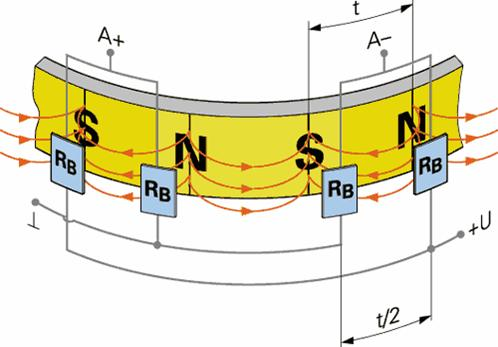
\includegraphics[width=7cm, height=6cm] {lenkdrehmomentsensor.png}
								\caption {\cite{TS13}: Abbildung: magnetoresistives Prinzip}
							\end{figure}			 

	
					\item 2. Optisches Prinzip:

							Vor und hinter dem Torsionsstab ist jeweils eine Scheibe angebracht, welche eine bestimmte Codierung mittels eingelassenen Löchern haben.\\
							Zur Bestimmung der Einlenkgeschwindigkeit wird axial und parallel zu dem Torsionsstab eine Leuchtdiode (über der ersten Scheibe) und eine Fotodiode (unter der zweiten Scheibe) angebracht. \\
							Hierbei sendet die Leuchtdiode ein gebündeltes Licht aus, welches auf der gegenüberliegenden Seite von der Fotodiode erkannt wird. Bei einfallendem Licht verändert sich der durchfließende elektrische Strom durch die Fotodiode.\\
							Dreht sich also die Scheibe kommt es zu einem Wechsel der Stromstärke. Diese Impulse werden an das angebundene Steuergerät gesendet, welches aus diesen empfangenden Informationen die Berechnungen durchführt.\\
							(Fig. 7)
							\begin{figure}
								\centering
								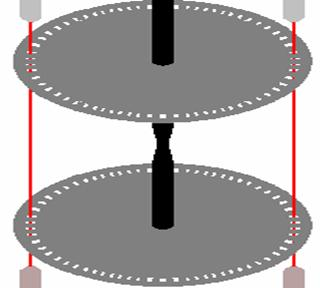
\includegraphics[width=7cm, height=6cm] {photoelektrisch.png}
 								\caption {\cite{TS14}: Abbildung: photooptisches Prinzip}
							\end{figure}	

				\end{itemize}

			\subsubsection{Regensensor}
				Dieser nicht- mechanische Sensor "[...] registriert Wassertropfen auf der Windschutzscheibe durch opto-elektrisches Verfahren." \cite{TS15}\\
				Der Sensor befindet sich innerhalb des Wischbereichs des Scheibenwischers, weshalb die Stärke des Regens/ Niederschlags wahrgenommen werden kann.\\
				In dem Sensor befindet sich eine Leuchtdiode und eine Fotodioden welche in einem bestimmten Abstand voneinander angebracht sind. Die Leuchtdiode sendet ein Infrarotlicht aus. Dieses Lichtbündel wird bei trockener Windschutzscheibe an der äußeren Scheibe reflektiert und nahezu mit voller Lichtstärke von dem Sensor aufgenommen. In der Physik spricht man hier von einer Totalreflexion.\\
				Befinden sich nun Wassertropfen in dem Bereich des Sensors auf der Frontscheibe wird durch den dort sich drauf befindlichen Wassertropfen das ausgesendete Lichtbündel nicht komplett reflektiert, sondern ein Teil des Lichtes wird gebrochen und durch den Tropfen gestreut. Das Resultat daraus ist, dass der ausgesendete Lichtstrahl nur noch mit einem Bruchteil der ursprünglichen Stärke den Sensor erreicht.\\
				Aus diesen Daten errechnet die dort darin befindliche Elektronik die Stärke des Niederschlages, gibt diese an ein Steuergerät weiter, welches wiederum die Scheibenwischer ansteuert. Somit bleibt die Oberfläche des Sensors immer tropfenfrei und es wird ein optimales Messergebnis erreicht. (Fig. 8)
				
				\begin{figure}
					\centering
					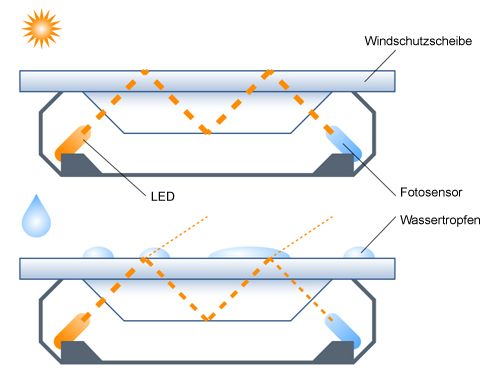
\includegraphics[width=10cm, height=8cm] {regensensor.png}
					\caption {\cite{TS16}: Abbildung: Regensensor Prinip}
				\end{figure}	
			
			\subsubsection{Seitenwandtorsionssensor}
				Im Folgenden Abschnitt wird der Seitenwandtorsionssensor mit SWT ( engl.: Sidewall Torsion Sensor) abgekürzt.\\ 
				Elektronische Regelsysteme wie ABS oder ESP benötigen sämtliche Informationen über das Zusammenspiel zwischen Fahrzeug und dem Fahruntergrund und den daraus entstehenden Kräften. Um die einzelnen Sekundärgrößen wie Motorleistung, Bremsdruck, Radgeschwindigkeit und Fahrzeugbeschleunigung zur Berechnung nicht mehr benutzen zu müssen, wurde von Continental ein Sensorsystem entwickelt, welches das Rad als Sensor fungieren lässt, das sogenannte SWT-System. 
				
				\begin{figure}
					\centering
					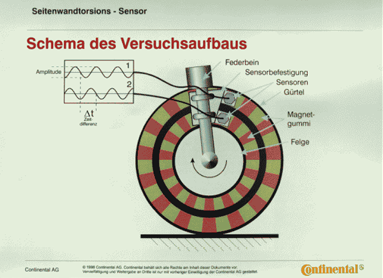
\includegraphics[width=10cm, height=7.5cm] {swt1.png}
					\caption {\cite{TS17}: Abbildung: Reifen als Sensor}
				\end{figure}
			
				(Fig. 9)Der Reifen besteht aus Magnetgummi und den Magnetfeldsensoren, sowie einem Signalaufbereitungssystem und einer zentralen Recheneinheit.\\
				Um die Funktionsweise verstehen zu können müssen erst einige Begriffe erörtert werden:
				
				\begin{itemize}
					\item Beschleunigen: Die Art des Kraftaufwandes, welche zum Bewegen des Fahrzeuges benötigt wird.
					\item Bremsen: Eine negative Beschleunigung, die entgegengesetzt der Fahrtrichtungsbeschleunigung, und somit mit entgegengesetzter Kraft wirkt.
					\item Längskräfte: Die Kräfte, welche beim Beschleunigen oder Bremsen auf den Reifen wirken.
					\item Querkräfte: Die Kräfte, welche "[...]quer zur Fahrrichtung wirken und bei Kurvenfahrt auftreten[...].\cite{TS18} Wird oftmals auch als Seitenkraft (S) bezeichnet.
					\item Verformung: Der Reifen wird durch die einwirkenden Kräfte aus seiner ursprünglichen Form gebracht und somit verformt sich dieser. Nachdem die einwirkende Kraft nachlässt, formt sich der Reifen wieder zurück in eine ursprüngliche Form.
					
					\begin{figure}
						\centering
						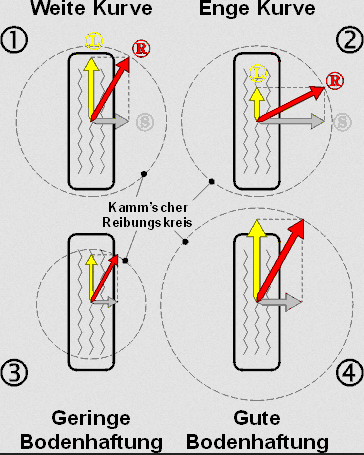
\includegraphics[width=5cm, height=7cm] {l_qkraft.png}
						\caption {\cite{TS19}: Abbildung: Zusammenspiel zwischen Längs- und Querkraft}
					\end{figure}
					
					\begin{flushleft}
						Hierbei ist der gelbe Pfeil (L) die Längskraft, also die Beschleunigung des Fahrzeuges.
						Der graue Pfeil entspricht der Querkraft (S) und der rote Pfeil ist die tatsächlich übertragene Kraft auf den Fahruntergrund.\\ (Fig. 10)
					\end{flushleft}
					  
				\end{itemize}
			
				\begin{flushleft}
					
					Die Messung findet mittels der Verformung statt. Hierfür werden zwei Sensoren am Fahrwerk angebracht, wobei einer der beiden auf der Höhe der Felge ist und der andere nahe am Scheitelpunkt des Reifens angebracht wird. Darüber hinaus ist die Reifenseitenwand magnetisch, um ein Messergebnis erzielen zu können.\\
					In der obrigen Abbildung erkennen wir ein Muster auf dem Reifen. Dies ist darauf zurückzuführen, dass ein Magnetpulver in die Reifenseitenwand eingemischt wird. Dieses Gemisch wird über den gesamten Umfang des Reifens gestrichen und somit erhält man eine Abwechslung zwischen Nordpol und Südpol Die Streifen stellen dies bildlich dar.\\
					Solange auf den Reifen keine Längskräfte wirken, "[...] erfolgt der Wechsel zwischen den Magnetpolen an beiden "Sensoren gleichzeitig, die ZEitdifferenz zwischen den Signalen beider Sensoren ist Null."\cite{TS20} \\
					Beschleunigt oder Verzögert der Fahrer das Fahrzeug, überschreiten die Grenzen der Magnete zu unterschiedlichen Zeiten die Sensoren, somit ist eine Zeitdifferenz zu messen. Diese gemessene Zeitdifferenz wird an ein eingebautes Steuergerät gesendet, welche die Fahrassistenzsysteme wie ASR und ABS anspricht und dementsprechend der derzeitigen Fahrsituation anpasst.\\
					Während einer Kurvenfahrt kann der Abstand zwischen der Reifenseitenwand und dem Sensor gemessen, da sich mechanisch gesehen der Abstand zwischen diesen verkürzt/ vergrößert wird und somit ändert sich ebenfalls die Stärke des Magnetfelds.\\
					Mit Hilfe diesen gemessenen Werten können Hilfssysteme wie ASB und ESP entsprechend angesteuert werden. Dies sorgt für ein sichereres, da die Ansteuerung optimiert werden kann. In der Praxis bedeutet dies, dass der Fahrer einen kürzeren Bremsweg und eine bessere Kontrolle auf kurvenreichen und schweren Strecken über das Fahrzeug hat.
					
				\end{flushleft}
				
			\subsubsection{Reifensensor}
				Ein in den Reifenprofil eingebetteter Chip überträgt hochfrequent die Signale an eine im Radkasten befindliche Antenne und wird von dieser ausgelesen. Ändert sich der Zustand der Straße verändert der Sensor das Signal. Dies geschieht pro Sekunde mehrere Male. Darüberhinaus kontrolliert der Sensor permanent den Reifendruck. Mit diesen Informationen kann nicht nur die Lebensdauer des Reifens, sondern auch die Sicherheit erhöht werden, da sich gezielt ABS und ESP einschalten.\\(Fig. 11)
				
				\begin{figure}
					\centering
					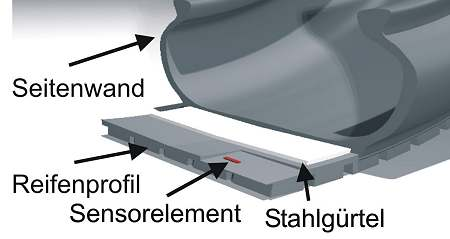
\includegraphics[width=7cm, height=5cm] {reifensensor.png}
					\caption {\cite{TS19}: Abbildung: Einpflanzung des Chips in den Reifen}
				\end{figure}
			
			
			\subsubsection{Reifendrucküberwachungssystem(RDKS)}
				RDKS (engl.: TMPS (Tire Pressure Monitoring System)) wird eingesetzt, um die Lebensdauer des Reifens zu erhöhen. Am 1. November 2014 die Reifen- und Autohersteller verpflichtet, ein RKDS zu implementieren. Hierbei wird jeder Reifen mit einem Sensor ausgestattet, damit der Fahrer Luftverlust des Reifens oder gar einen Plattfuß bemerken kann.\\
				in der folgenden Tabelle (Table 2) sind prinzipiell zwei Ausführungen des Sensors aufgelistet:
				
				\begin{table}	
					\begin{tabular}{c|c|c}
						
						\textbf {  } & \textbf{Passiv} & \textbf {Aktiv}\\
						
						
						\hline
						\textbf{Erklärung:} & Platter Reifen hat einen kleineren Abrollumfang und dreht sich schneller.\\&ABS Sensoren messen dies und das Steuergerät erkennt dies & Jeder Reifen besitzt eigenen Sensor und sendet Informationen über Druck und Temperatur per Funkt an Steuergerät.\\
						
						
						\hline
						\textbf{Vorteil:} & kostengünstig, in Kombination mit Ruflat Tyre eine optimale Lösung, \\&da nur eine geänderte Software und Kontrolle erforderlich sind. & Exakte Messung und ab einer Differenz von 0,2 Bar wird ein Alarm ausgelöst. Reserverad wird mit überwacht.\\
						
	
						\hline
						\textbf{Nachteil:} & schleichender Luftverlust der Räder an einer Achse wird nicht erkannt.\\&Differenzen nur von größer 0,5 Bar werden nur während der Fahrt erkannt.\\&  Höherer Spritverbrauch durch zu niedrigen Luftdruck. & Teuer für Reifenmontage, da Reifen kodiert werden müssen und der Reifenwechsel aufwendig wird.\\
						\hline
					
					\end{tabular}
				\caption{ \cite{TS22}: Tabelle Eingleiderung Aktiv und Passiv}
				\end{table}	
			
			
				\begin{flushleft}
						
					Die Reifenelektronik sitzt auf der Innenseite des Reifen und misst in kurzen definierten Zeitabständen Reifendruck und Temperatur. Jeder Sensor ist mit einer eigenen ID- Nummer ausgestattet. Per Funkt werden die Daten an die eigene Empfangsstation Datenpakete geschickt, welche die ID, sowie Druck und Temperatur des Reifens beinhalten. Dieses Empfangsgerät sendet die empfangenen Daten kabelgebunden weiter an das Steuergerät. Dieses wertet die Daten aus und sendet bei Bedarf, sprich Unter- oder Überschreitung einer der Daten, eine Meldung an die Kontrollanzeige. (Fig. 12)
					
				\end{flushleft}	
				
				\begin{figure}
					\centering
					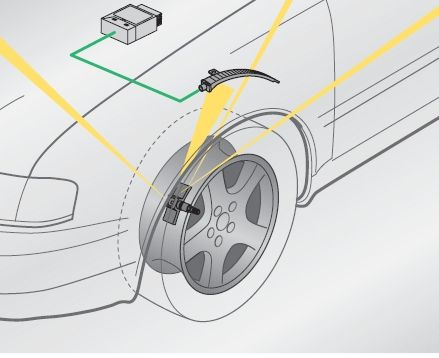
\includegraphics[width=7cm, height=5cm] {rdks.png}
					\caption {\cite{TS23}: Abbildung: Einpflanzung des Chips in den Reifen}
				\end{figure}
				
			\subsubsection{Hallsensor}
				Einsatz von dem Hallsensor sind: 
				\begin{itemize}
					\item Zündanlage
					\item Getriebeausgabedrehzahl
					\item Radlöseerkennung/- warunung (Audi)
					\item aktiver Drehzahlsensor in ABS- Bremsanlagen
					\item Nockenwelle (Koordination von Eispritzbeginnberechnung oder Pumpe-Düse, sowie Klopfregelung)
				\end{itemize}
				
				Am letzteren wird im Folgenden die Funktion des Sensors beschrieben.\\
				Die Nockenwelle bringt einen aus ferromagnetischem Material angefertigten Rotor zum Drehen. Zwischen Rotor und einem Dauermagnet befindet sich der Sensor. Durch den Dauermagneten wird ein Magnetfeld erzeugt, welches den Sensor senkrecht durchfließt. Passiert ein metallischer Gegenstand, beispielsweise ein Zahn der Nockenwelle, verändert dieser das Magnetfeld, welches den Sensor durchfließt.
				Elektronen werden senkrecht zum Magnetfeld stärker abgelenkt, wobei eine Hall-Spannung von mehreren Millivolt erzeugt. Eine integrierte Auswerteelektronik bereitet das Signal auf und leitet es an in Form eines Rechtecksignals an das Steuergerät geleitet.\\\cite{TS24}
				(Fig. 13)
				\begin{figure}
					\centering
					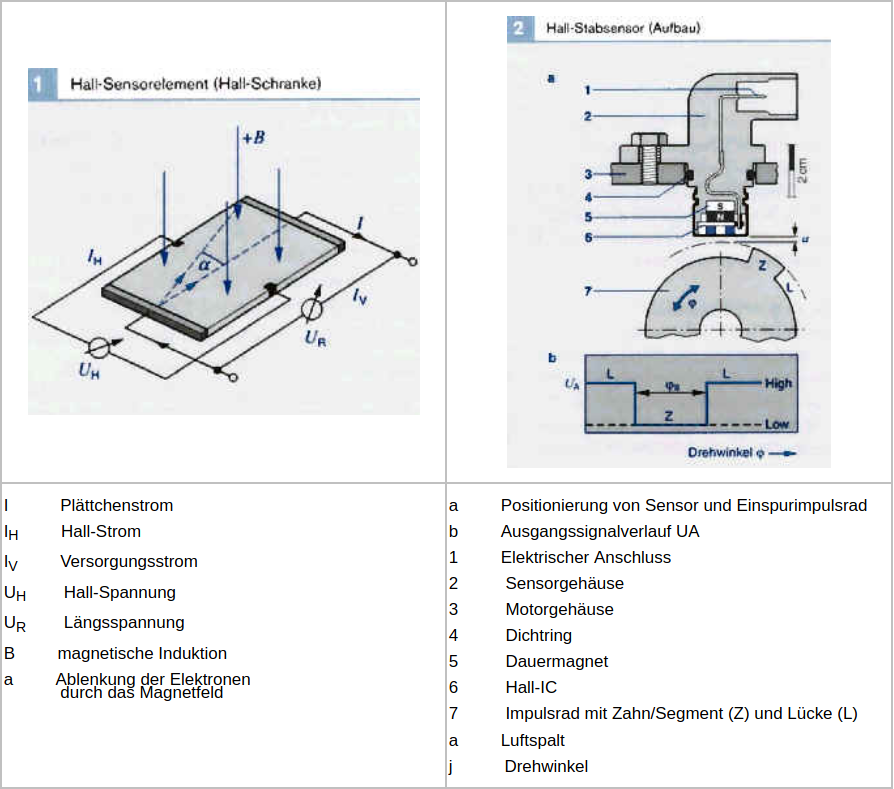
\includegraphics[width=7cm, height=5cm] {hall.png}
					\caption {\cite{TS25}: Abbildung: Aufbau des Hall- Sensors}
				\end{figure}
			
			
			\subsubsection{Rad- Drehzahlsensor}
			
				Dieser Sensor arbeitet auf dem Hall- Prinzip: (Fig. 14)
				\begin{figure}
					\centering
					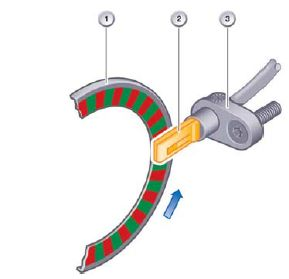
\includegraphics[width=7cm, height=5cm] {radsensor.png}
					\caption {\cite{TS26}: Abbildung: Aufbau des Sensors}
				\end{figure}
			
				\begin{flushleft}
					Durch drei entsprechend angeordneten Sensoren kann die Drehrichtung des Rades erkannt werden. Ein entsprechend angeordneter Magnet (Fig.15) ersetzen hierbei die Funktion der mechanischen Zahnräder.\\
					Aktive Sensoren: Dieser wird bereits mit Spannung versorgt und erzeugt aus dem wechselnden Magnetfeld ein Rechtecksignal und sendet diese unverändert an ein Steuergerät.\\
					Dies ermöglicht ebenso eine Geschwindigkeitsmessung von 0,1km/h. Diese Werte kann man zum Beispiel für Einparksysteme oder Navigationssysteme benutzen.\cite{TS27}
					(Fig. 15)
				\end{flushleft}

				\begin{figure}
					\centering
					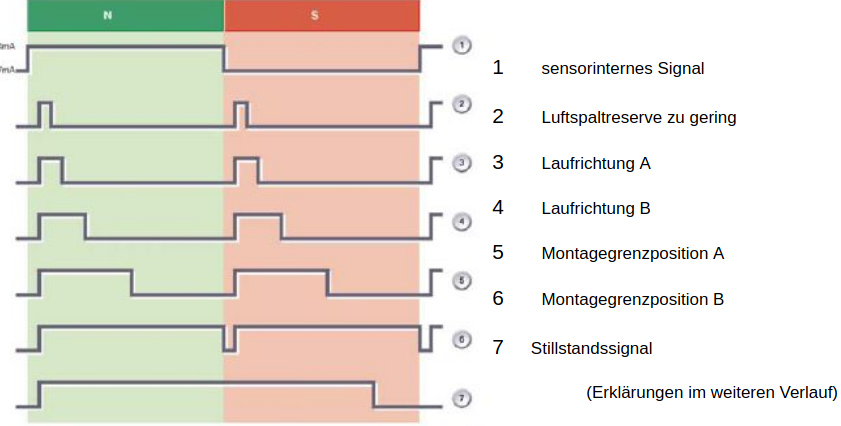
\includegraphics[width=7cm, height=5cm] {signalverlauf_hall.png}
					\caption {\cite{TS28}: Abbildung: Signalverlauf des Sensors}
				\end{figure}

			\subsubsection{Lambdasonden}
				Dies dient pinzipiel zum vollständingen und ordnungsgemäßen Verbrennen des Luft-Kraftstoffgemisches. Das Verhältnis zwischen Luft und Kraftstoff wird als Lambdawert (=$\lambda$)bezeichnet.\\
				$\lambda = 1$ heißt also, dass die zugeführte Luftmenge dem theoretischen Luftbedarf entspricht."\cite{TS29}\\
				Herrscht ein Luftmangel ($\lambda$ ca 0.9, festes Gemisch) hat der Motor seine beste Leistung, herrscht Luftüberschuss ($\lambda$=1.1, mageres Gemisch) hat man den niedringsten Verbrauch.\\
				Zur Regelung der Gemischzusammensetzung wird die Abgaszusammensetzung mit Hilfe der Lambdasonde gemessen, welche erkennen, ob diese zu fettig oder zu mager sind. Es misst den Restsauerstoff, welcher nach der Verbrennung übrig bleibt. (Fig. 16)		
			
				\begin{figure}
					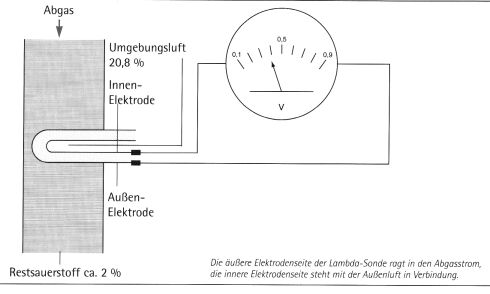
\includegraphics[width=7cm, height=5cm] {lambdasonde.png}
					\caption {\\\cite{TS30}: Abbildung: Messprinzip von Lambdasonde}
				\end{figure}
			
				\begin{flushleft}
					Der Sauerstoffgehalt der Außenluft dient als Referenzwert. Dieser Wert wird mit dem Restsauerstoffgehalt der Abgase vergleichen. Die Sonde besteht aus einem Spezialkeramikkörper, deren Oberfläche gasduchlässig ist. Der äußere Teil der Sonde steht mit dem Abgas in Verbindung, der innere beinhaltet frische Außenluft.\\
					Die Sonde arbeitet nach dem Galvanischen Prinzip, nur dass sie keinen flüssigen sondern einen festen Elektrolyten besitzt. Ab einer Temperatur von etwa 350°C lässt der Keramikkörper den Sauerstoff durch, sperrt jedoch den Durchlass für Elektronen.
					
					Sauerstoff ist im gasförmigen Zustand elektrisch neutral und der Festkörper lässt allerdings nur Sauerstoffione passieren. Somit muss der Sauerstoff an der Referenzelektrode negativ aufgeladen werden, an der Messelektrode wieder entladen werden.
					
					Durch die aufgenommenen Elektronen bildet sich auf der Innenseite der Sonde ein Elektronenüberschuss und auf der Außenseite ein Elektronenmangel, also insgesamt eine elektrische Spannung. Diese wird über Leitungen zur Auswertung zum Steuergerät geleitet."\cite{TS31}
				\end{flushleft}
			
			\subsubsection{Airbagsensor}
					Zum Auslösen des Airbags werden mehrere Frontsensoren verwendet, welche an diversen Stellen im Auto angebracht sind. Die Beschleunigungssensoren messen einwirkende Kräfte und geben ein Signal an das Steuergerät. Damit der Airbag nicht fälschlicher Weise geöffnet wird, muss ein Sicherheitssensor innerhalb des Steuergerätes dies bestätigen. "Durch das genau Erfassen der Unfallschwere wird die Auslösung der Airbags und der Gurtstraffer aktiviert."\cite{TS32}\\
					Faktoren sind: 
					
					\begin{itemize}
						\item Aufprallstärke
						\item sicherheitsgurte angelegt
						\item Sitzposition des Fahrers und Beifahrers
					\end{itemize}
				
				
				\subsubsection{Positionssensoren}
					Diese Sensoren sind an diversen relevanten Stellen des Automobils befestigt. Sie geben Aufschluss über die in der Nähe befindlichen Gegenstände.\\
					Um diese erkennen zu können wird ein Ultraschallsensor eingesetzt, welcher ein Signal aussendet. Falls ein Gegenstand in der Nähe ist, reflektiert dieser die Schallwellen und ein Ultraschallempfänger erhält diese. Durch die Zeitdifferenz des ausgesendeten und des erhaltenden Signals kann die Entfernung errechnet werden. Kommt das Objekt näher, so verkürzt sich der Abstand und somit auch die Zeit des Eintreffen des Schalls.\\
					Der Sensor sendet zu einen die Zeit, wann dieser die Ultraschallwellen gesendet hat und als nächsten Schritt die reflektierten Signale. Aus dieser Differenz kann über physikalische Formeln der Abstand zwischen Auto und Gegenstand errechnet werden. Nähert sich das Auto einem Objekt, so verkürzt sich die Zeit zwischen den austretenden und empfangenen Schallwellen. Bei dem kleinsten zulässigen Abstand meldet das Steuergerät dies der Kontrolleinheit und der Fahrer wird informiert.\\
					Falls sich kein Objekt in der Nähe befindet wird auch kein Signal reflektiert und somit erkennt das Steuergerät, dass keine Kollision stattfinden kann. (Fig. 17)
				
					\begin{figure}
						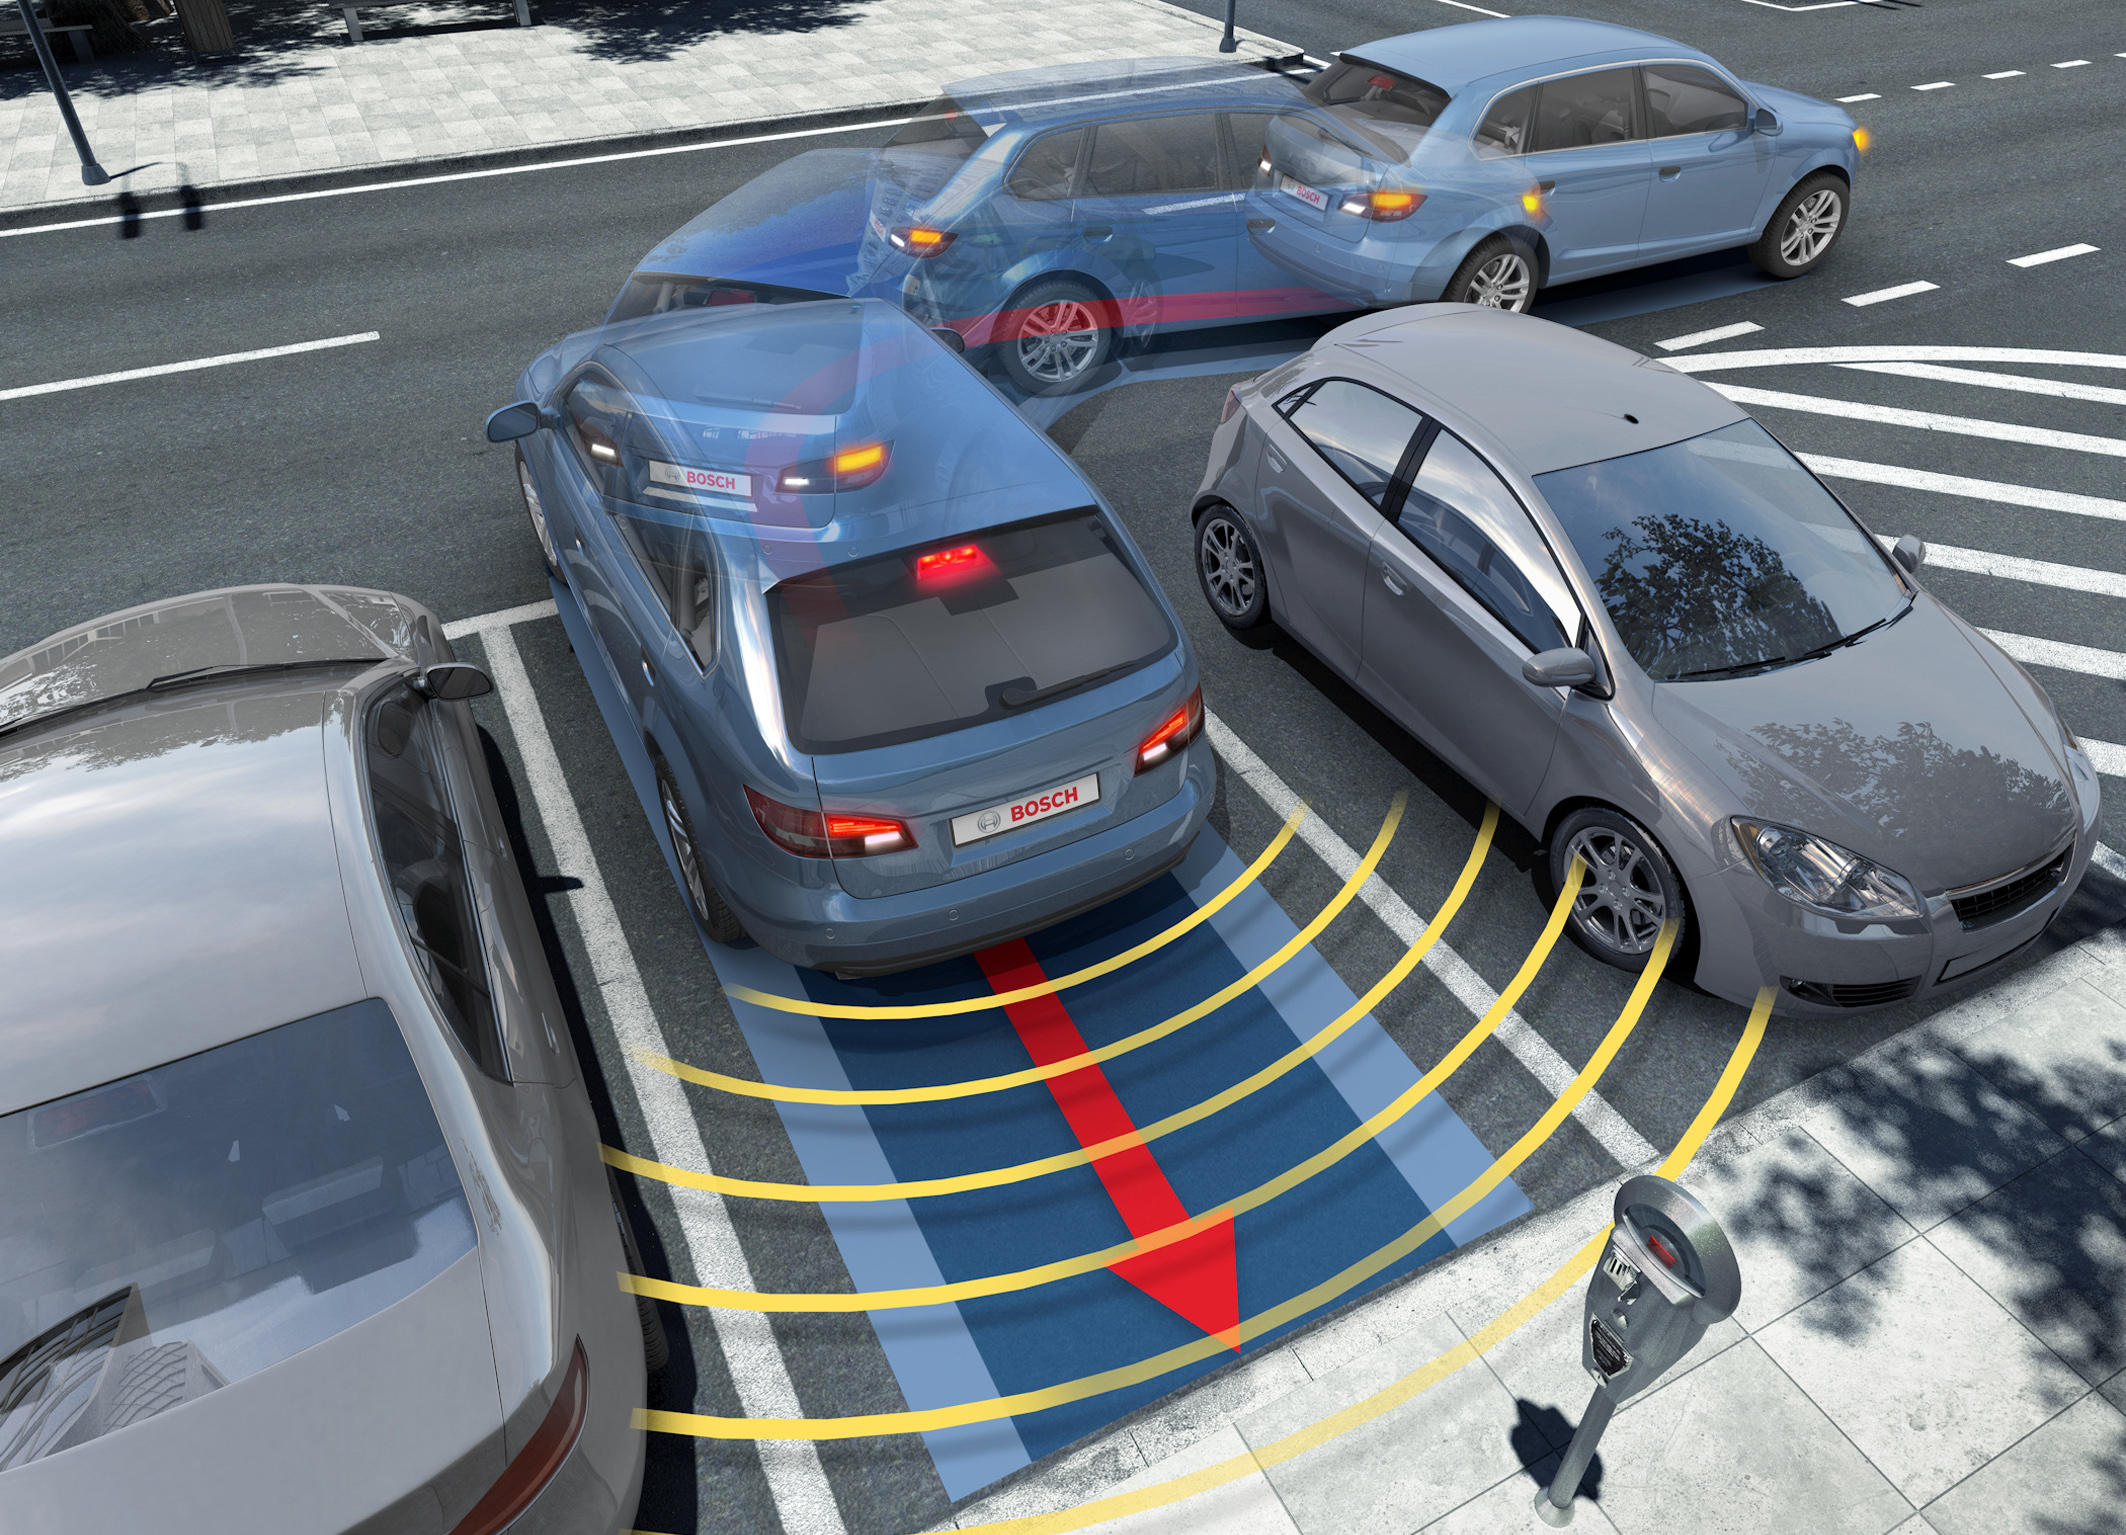
\includegraphics[width=7cm, height=5cm] {ultraschall.png}
						\caption {\\\cite{TS33}: Abbildung: Darstellung Ultraschallsensor}
					\end{figure}\\
					
				
				
		\subsection{Smarte Sensoren} 
			Unter smarten Sensoren versteht man, dass der eingebaute Sensor bereits schon eine eingebaute Recheneinheit und Logik integriert hat. Dieser kann neben dem eigentlichen Messen die eingelesenen Daten Verarbeiten und in diesem Zustand dem Steuergerät überreichen. Dies hat den Vorteil, dass das Steuergerät keine überflüssigen Rechenschritte abarbeiten muss und somit mehr Rechenleistung für das Reagieren auf besondere Ereignisse hat.\\
			Diese können beispielsweise mitunter bei Feldbussystemen wie LIN, CAN, FLEX RAY eingesetzt werden.		
		
		
		
		\subsection{Zukunftsvisionen} 
 			Durch das Weiterentwickeln der Sensortechnik können beispielsweise Unfälle vermieden werden, da der Sensor eine deutlich schnellere Reaktionszeit aufweisen als ein Mensch. Ein Beispiel wäre, das bestehende Positionssensorsystem durch eine neue Art der Messung zu ersetzte. Hierbei werden die Ultraschallsensoren durch so genannte Radarkameras ersetzt, welche einen deutlich weiteren Radius abdecken können, als die bisher herkömmlichen Sensoren.\\(Fig. 18)
 			
 			\begin{figure}
 				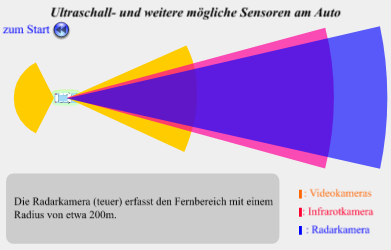
\includegraphics[width=7cm, height=5cm] {radarsensor.png}
 				\caption {\\\cite{TS34}: Abbildung: Unterschied: Video-, Infrarot- und Radarkamera}
 			\end{figure}

			\begin{flushleft}
							
				Hier kann man eindeutig den Unterschied der Reichweiten der einzelnen Sensoren sehen.\\
				
				Neben diesem Effekt kann man durch neue entwickelten Sensoren beispielsweise der Spritverbrauch und somit den Ausstoß an CO2 verringert werden.\\
				Auch im Hinblick auf Elektromobilität wird es neue Sensoren geben, welche zur Überwachung der Batterie eingesetzt werden muss, Ansteuerung der Räder usw.
				
			\end{flushleft} 

@Book{ 
	Bosch [TS01] 
	Konrad Reif: 		Sensoren im Kraftfahrzeug,
	Author		= 		Konrad Reif,
	Title		=		Sensoren im Kraftfahrzeug,
	Publisher	=		Springer Vieweg,
	Year		=		2012,
	Address		=		Wiesbaden,
	isbn 		= 		978-3-8348-1778-5,
	Series 		=		{Bosch Professional Automotive Information},
}
\\

@Internet{ Tabelle[TS02],
URL: https://www.itwissen.info/lex-images/uebersicht-ueber-verschiedene-sensoren.png}
\\

@Internet{ Information[TS03],
	URL: https://www.itwissen.info/lex-images/uebersicht-ueber-verschiedene-sensoren.png}
\\

@Internet{ Information[TS04],
	URL: https://www.kfztech.de/kfztechnik/elo/sensoren/ntc/ntc5.jpg}
\\

@Internet{ Information[TS05],
	URL: https://www.kfztech.de/kfztechnik/elo/sensoren/ntc.htm}
\\

@Internet{ Information[TS06],
	URL: https://www.kfztech.de/kfztechnik/elo/sensoren/ntc/thermoelement.jpg}
\\

@Internet{ Information[TS07],
	URL: https://www.channypicture.com/pic/UploadFile/P0/SKU229953/6BCD9366CB23CB6653FCD236366646D2999A8D6699D29D26839DD2C826469CCF16C899CA50CB16CC46A0CA.jpg}
\\

@Internet{ Information[TS09],
	URL:
https://www.kfztech.de/kfztechnik/elo/sensoren/induktivgeber.htm\
\\

@Internet{ Information[TS09],
	URL: https://www.kfztech.de/kfztechnik/elo/sensoren/induktiv/indukt2.jpg}
\\

@Internet{ Information[TS10],
	URL: https://www.kfztech.de/kfztechnik/elo/sensoren/oelsensor.htm}
\\

@Internet{ Information[TS11],
	URL:https://www.kfztech.de/kfztechnik/fahrwerk/lenkung/drehmosensor.htm}
\\

@Internet{ Information[TS12],
	URL: https://www.kfztech.de/kfztechnik/fahrwerk/lenkung/drehmosensor.htm}
\\

@Internet{ Information[TS13],
	URL: https://www.kfztech.de/kfztechnik/fahrwerk/lenkung/magnetroresistiv.jpg}
\\

@Internet{ Information[TS14],
	URL: https://www.kfztech.de/kfztechnik/fahrwerk/lenkung/photoelektrisch.jpg}
\\

@Internet{ Information[TS15],
	URL: https://www.kfztech.de/kfztechnik/sicherheit/regensensor.htm}
\\

@Internet{ Information[TS16],
	URL: https://archiv.langzeittest.de/volvo-s40/intern/grafik/cb-regensensor-prinzip.jpg}
\\

@Internet{ Information[TS17],
	URL: https://www.kfztech.de/kfztechnik/sicherheit/swt/swt1.gif}
\\

@Internet{ Information[TS18],
	URL: http://www.arstechnica.de/index.html?name=http://www.arstechnica.de/auto/differential/rad/seitenfuehrung.html}
\\

@Internet{ Information[TS19],
	URL: http://www.arstechnica.de/auto/differential/rad/kammscherkreis.gif}
\\

@Internet{ Information[TS20],
	URL: https://www.kfztech.de/kfztechnik/sicherheit/swt.htm}
\\

@Internet{ Information[TS21],
	URL: https://www.kfztech.de/kfztechnik/elo/sensoren/Reifensensor.jpg}
\\

@Internet{ Information[TS22],
	URL: https://www.kfztech.de/kfztechnik/fahrwerk/reifen/rdks.htm}
\\

@Internet{ Information[TS23],
	URL: https://www.kfztech.de/kfztechnik/fahrwerk/reifen/rdks/rdks_audi.jpg}
\\

@Internet{ Information[TS24],
	URL: https://www.kfztech.de/kfztechnik/elo/sensoren/hallsensor.htm}
\\

@Internet{ Information[TS25],
	URL: https://www.kfztech.de/kfztechnik/elo/sensoren/hall/hallse1.jpg}
\\

@Internet{ Information[TS26],
	URL: https://www.kfztech.de/kfztechnik/elo/sensoren/drehzahl/radsensor_aktiv1.jpg}
\\

@Internet{ Information[TS27],
	URL: https://www.kfztech.de/kfztechnik/elo/sensoren/drehzahlsensor.htm}
\\

@Internet{ Information[TS29],
	URL: https://www.kfztech.de/kfztechnik/motor/abgas/lambda/lambda1.htm}
\\

@Internet{ Information[TS30],
	URL: https://www.kfztech.de/kfztechnik/motor/abgas/lambda/messprinzip1.jpg}
\\

@Internet{ Information [TS31],
	URL: https://www.kfztech.de/kfztechnik/motor/abgas/lambda/lambda1.htm}
\\

@Internet{ Information [TS32],
	URL: https://www.kfztech.de/kfztechnik/sicherheit/airbag/airbag.htm}
\\

@Internet{ Information [TS33],
	URL: https://www.bosch-presse.de/pressportal/de/media/migrated_media/pressegespr_ch_fahrerassistenz_2012/1-ae-17866-2.jpg}
\\

@Internet{ Information [TS34],
	URL: https://www.leifiphysik.de/akustik/schallgeschwindigkeit/ausblick/ultraschall-beim-auto}



